\documentclass[11pt]{article}
\usepackage[margin=1cm]{geometry}
\usepackage{amsmath,amssymb}
\usepackage{xcolor}
\usepackage{tikz}
\usetikzlibrary{arrows.meta, positioning, calc, shadows.blur, decorations.pathreplacing, decorations.markings, backgrounds}

% ---------- Palette moderne ----------
\definecolor{grayTop}{RGB}{190,190,190}
\definecolor{grayBot}{RGB}{110,110,110}
\definecolor{greenTop}{RGB}{190,205,120}
\definecolor{greenBot}{RGB}{90,110,55}
\definecolor{redTop}{RGB}{235,175,160}
\definecolor{redBot}{RGB}{195,90,80}
\definecolor{goldTop}{RGB}{235,200,120}
\definecolor{goldBot}{RGB}{150,150,150}
\definecolor{accentRed}{RGB}{200,30,30}
\definecolor{accentBlue}{RGB}{20,60,190}

% ---------- Styles communs ----------
\tikzset{
  databox/.style={
    rectangle, rounded corners=6pt, draw=black!60, thick,
    minimum width=2.4cm, blur shadow={shadow blur steps=6, shadow xshift=1pt, shadow yshift=-1.5pt},
    align=center, font=\large, text=black!85
  },
  grayfill/.style={top color=grayTop, bottom color=grayBot},
  greenfill/.style={top color=greenTop, bottom color=greenBot},
  redfill/.style={top color=redTop, bottom color=redBot},
  goldfill/.style={top color=goldTop, bottom color=goldBot},
  whitebox/.style={rectangle, draw=black, thick, rounded corners=2pt,
    minimum width=3cm, minimum height=1.2cm, align=center, font=\normalsize},
  bigarrow/.style={-{Latex[length=3mm,width=2.5mm]}, thick, draw=black!80},
  label/.style={font=\small\bfseries, align=center},
  bluelabel/.style={font=\small\bfseries, text=accentBlue, align=center},
  redlabel/.style={font=\small\bfseries, text=accentRed, align=center}
}

\begin{document}

%======================================================
% FIGURE 1 : ConsID
%======================================================
\begin{figure}[htbp]
\centering
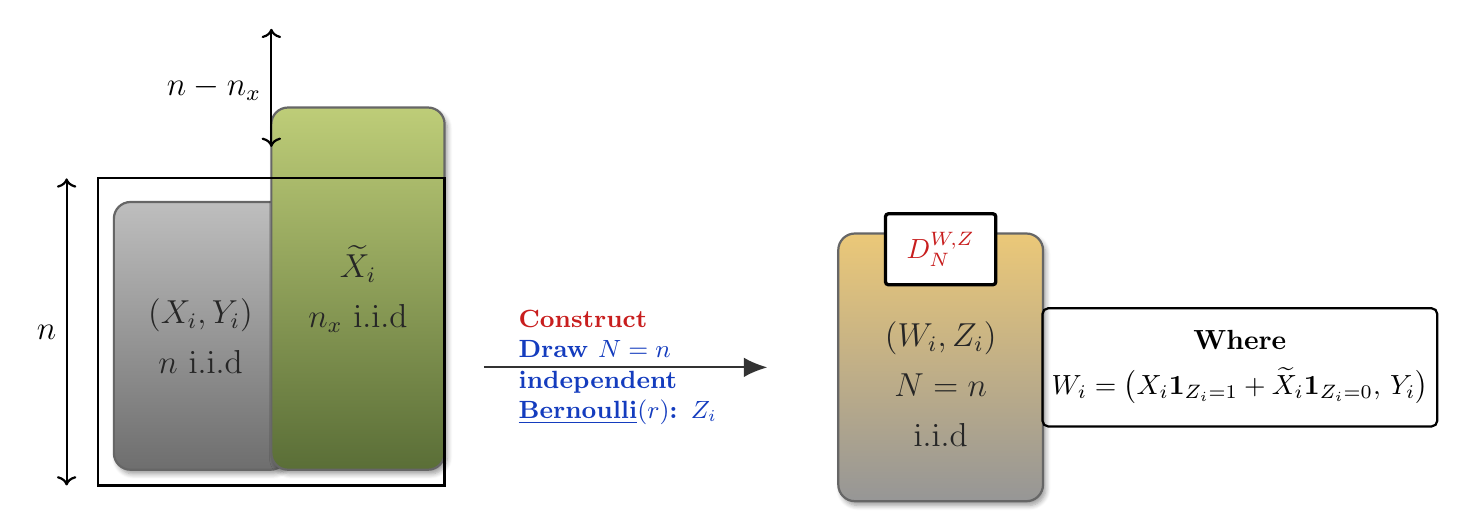
\begin{tikzpicture}[scale=1]

% --- Boîte grise (X_i,Y_i) ---
\node[databox, grayfill, minimum height=3.4cm, minimum width=2.2cm] (XY) at (0,0)
  {$(X_i,Y_i)$\\[4pt] $n$ i.i.d};

% --- Boîte verte X tilde, décalée vers le haut et vers la droite (chevauchement) ---
\node[databox, greenfill, minimum height=4.6cm, minimum width=2.2cm] (Xt) at (2.0,0.6)
  {$\widetilde{X}_i$\\[4pt] $n_x$ i.i.d};

% --- Cadre noir englobant (n) ---
\draw[black, thick] (-1.3,-1.9) rectangle (3.1,-1.9+3.9);

% --- Flèches de cotation ---
\draw[<->,thick] (-1.7,-1.9) -- (-1.7,-1.9+3.9) node[midway,left,font=\large] {$n$};
\draw[<->,thick] (0.9,2.4) -- (0.9,3.9) node[midway,left,font=\large]{$n-n_x$};

% --- Flèche "Construct" ---
\node[bluelabel, align=left] (constructlabel) at (5.3,-0.4)
  {\textcolor{accentRed}{\textbf{Construct}}\\
   \textcolor{accentBlue}{Draw $N=n$}\\
   \textcolor{accentBlue}{independent}\\
   \textcolor{accentBlue}{\underline{Bernoulli}$(r)$: $Z_i$}};
\draw[bigarrow] (3.6,-0.4) -- (7.2,-0.4);

% --- Boîte D_N^{W,Z} dorée ---
\node[databox, goldfill, minimum height=3.4cm, minimum width=2.6cm] (DWZ) at (9.4,-0.4)
  {\phantom{x}\\[2pt] $(W_i,Z_i)$\\[4pt] $N=n$\\[4pt] i.i.d};
\node[draw=black, very thick, rounded corners=1pt, fill=white,
      minimum width=1.4cm, minimum height=0.9cm] (label1) at (9.4,1.1)
  {\textcolor{accentRed}{$\mathscr{D}_N^{W,Z}$}};

% --- Boîte "Where" ---
\node[whitebox, minimum width=4.6cm, minimum height=1.5cm] (where1) at (13.2,-0.4)
  {\textbf{Where}\\[4pt]
   $W_i=\big(X_i\mathbf{1}_{Z_i=1}+\widetilde{X}_i\mathbf{1}_{Z_i=0},\,Y_i\big)$};

\end{tikzpicture}
\caption{Construction I.D. (ConsID)}
\end{figure}

%======================================================
% FIGURE 2 : ConsIID (échange sur Y)
%======================================================
\begin{figure}[htbp]
\centering
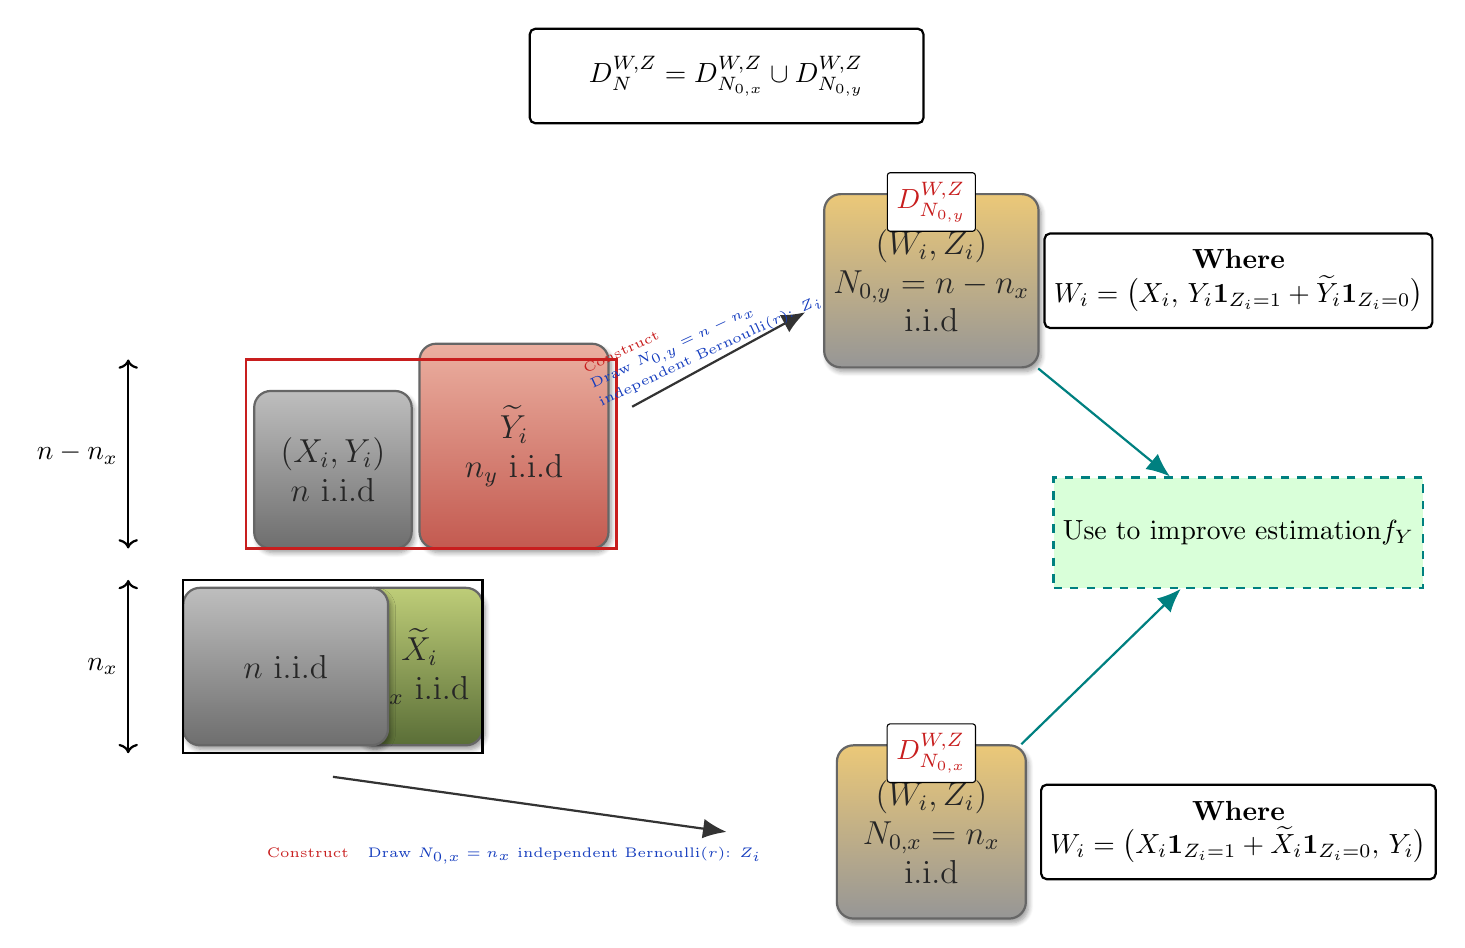
\begin{tikzpicture}[scale=1]

% --- Boîte englobante n (X,Y) + Y tilde, en haut ---
\node[databox, grayfill, minimum height=2.0cm, minimum width=2.0cm] (XY) at (0,1.0)
  {$(X_i,Y_i)$\\ $n$ i.i.d};
\node[databox, redfill, minimum height=2.6cm, minimum width=2.4cm] (Yt) at (2.3,1.3)
  {$\widetilde{Y}_i$\\ $n_y$ i.i.d};
\draw[accentRed, thick] (-1.1,0.0) rectangle (3.6,2.4);

% --- Boîte X tilde, en bas ---
\node[databox, greenfill, minimum height=2.0cm, minimum width=1.6cm] (Xt) at (1.1,-1.5)
  {$\widetilde{X}_i$\\ $n_x$ i.i.d};
\node[databox, grayfill, minimum height=2.0cm, minimum width=2.6cm] (XY2) at (-0.6,-1.5)
  {$n$ i.i.d};
\draw[black, thick] (-1.9,-2.6) rectangle (1.9,-0.4);

% --- Cotations ---
\draw[<->,thick] (-2.6,0.0) -- (-2.6,2.4) node[midway,left]{$n-n_x$};
\draw[<->,thick] (-2.6,-2.6) -- (-2.6,-0.4) node[midway,left]{$n_x$};

% --- Flèche Construct 1 (haut, vers D_{N0y}) ---
\draw[bigarrow] (3.8,1.8) -- (6.0,3.0);
\node[bluelabel, font=\tiny, align=left, rotate=25] at (4.7,2.7)
  {\textcolor{accentRed}{Construct}\\ \textcolor{accentBlue}{Draw $N_{0,y}=n-n_x$}\\ \textcolor{accentBlue}{independent Bernoulli$(r)$: $Z_i$}};

\node[databox, goldfill, minimum height=2.2cm, minimum width=2.4cm] (D0y) at (7.6,3.4)
  {$(W_i,Z_i)$\\ $N_{0,y}=n-n_x$\\ i.i.d};
\node[draw, fill=white, rounded corners=1pt] at (7.6,4.4) {\textcolor{accentRed}{$\mathscr{D}_{N_{0,y}}^{W,Z}$}};
\node[whitebox, minimum width=4.6cm] at (11.5,3.4)
  {\textbf{Where}\\ $W_i=\big(X_i,\,Y_i\mathbf{1}_{Z_i=1}+\widetilde{Y}_i\mathbf{1}_{Z_i=0}\big)$};

% --- Flèche Construct 2 (bas, vers D_{N0x}) ---
\draw[bigarrow] (0.0,-2.9) -- (5.0,-3.6);
\node[bluelabel, font=\tiny, align=left] at (2.3,-3.9)
  {\textcolor{accentRed}{Construct}\quad \textcolor{accentBlue}{Draw $N_{0,x}=n_x$ independent Bernoulli$(r)$: $Z_i$}};

\node[databox, goldfill, minimum height=2.2cm, minimum width=2.4cm] (D0x) at (7.6,-3.6)
  {$(W_i,Z_i)$\\ $N_{0,x}=n_x$\\ i.i.d};
\node[draw, fill=white, rounded corners=1pt] at (7.6,-2.6) {\textcolor{accentRed}{$\mathscr{D}_{N_{0,x}}^{W,Z}$}};
\node[whitebox, minimum width=4.6cm] at (11.5,-3.6)
  {\textbf{Where}\\ $W_i=\big(X_i\mathbf{1}_{Z_i=1}+\widetilde{X}_i\mathbf{1}_{Z_i=0},\,Y_i\big)$};

% --- Boîte d'union en haut ---
\node[whitebox, minimum width=5cm] at (5,6.0)
  {$\mathscr{D}_N^{W,Z}=\mathscr{D}_{N_{0,x}}^{W,Z}\cup \mathscr{D}_{N_{0,y}}^{W,Z}$};

% --- Boîte finale "Use to improve estimation" ---
\node[rectangle, draw=teal, dashed, thick, fill=green!15,
      minimum width=4cm, minimum height=1.4cm] (use) at (11.5,0.2)
  {Use to improve estimation\\ $f_Y$};
\draw[bigarrow, teal] (D0y) -- (use);
\draw[bigarrow, teal] (D0x) -- (use);

\end{tikzpicture}
\caption{Construction I.I.D. (ConsIID)}
\end{figure}

\end{document}